\chapter{Theoretical Background}\label{chap:01}

\section{LHCb}

\begin{figure}[H]
    \centering
    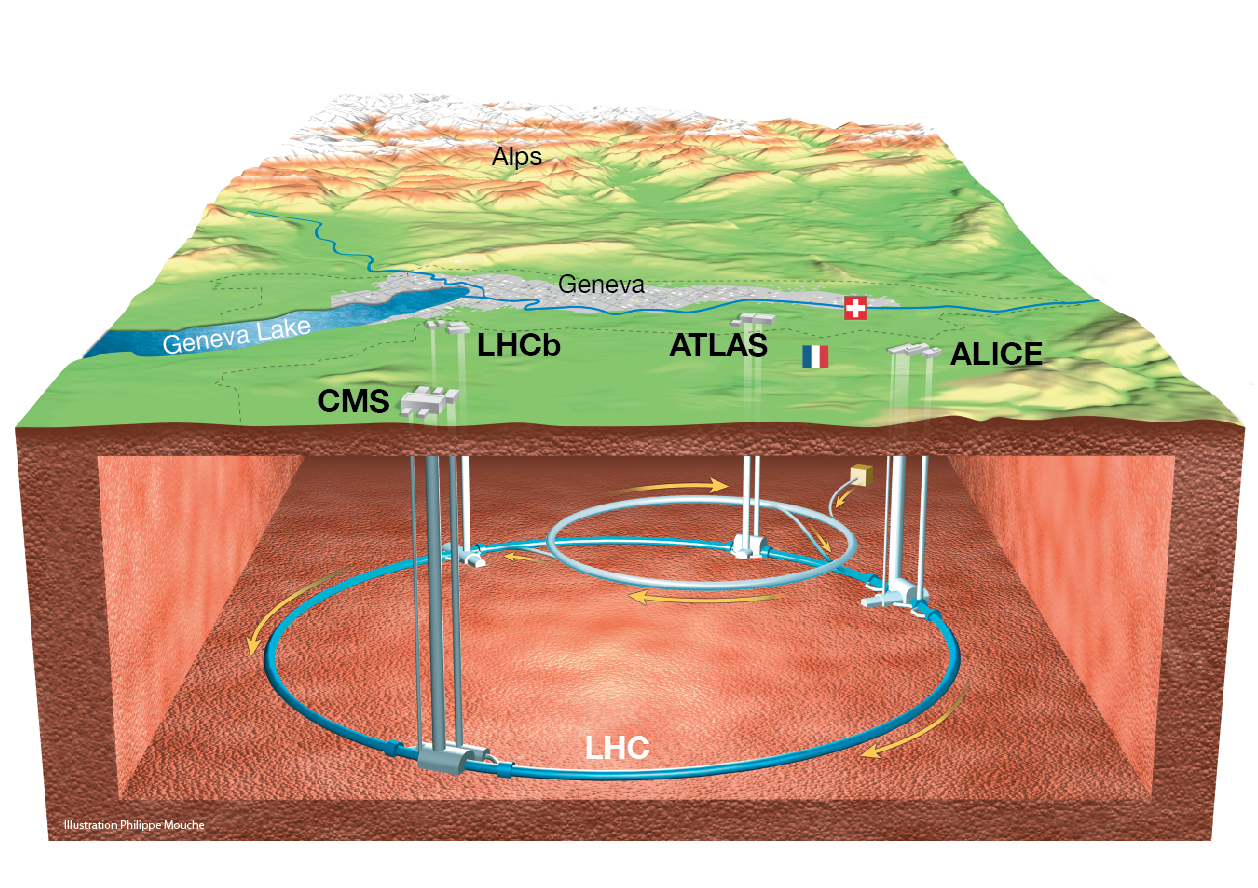
\includegraphics[width=0.7\linewidth]{images/LHC_scheme.png}
    \caption{LHC schema with ALICE, Atlas, CMS and LHCb at CERN.}
    \label{LHC}
\end{figure}

The LHCb Detector is part of one of the four large experiments set up on different points of the circular accelerator design of LHC, at CERN. Our detectors are constructed around collision points where the accelerated beams of protons are crossed with each other \( 40 \times 10^{16} \) times per second. Unlike rest of the detectors at LHC, the LHCb detector is a single arm forward spectrometer; meaning it is purpose built to detect particles from a singular direction. It can detect particles coming from the interaction point in the pseudorapidity range between 2 < η < 5 and it is design philosophy is geared towards measuring b (bottom) and c (charm) hadron properties alongside CP violation. \cite{LHCb_detector}


\begin{figure}[H]
    \centering
    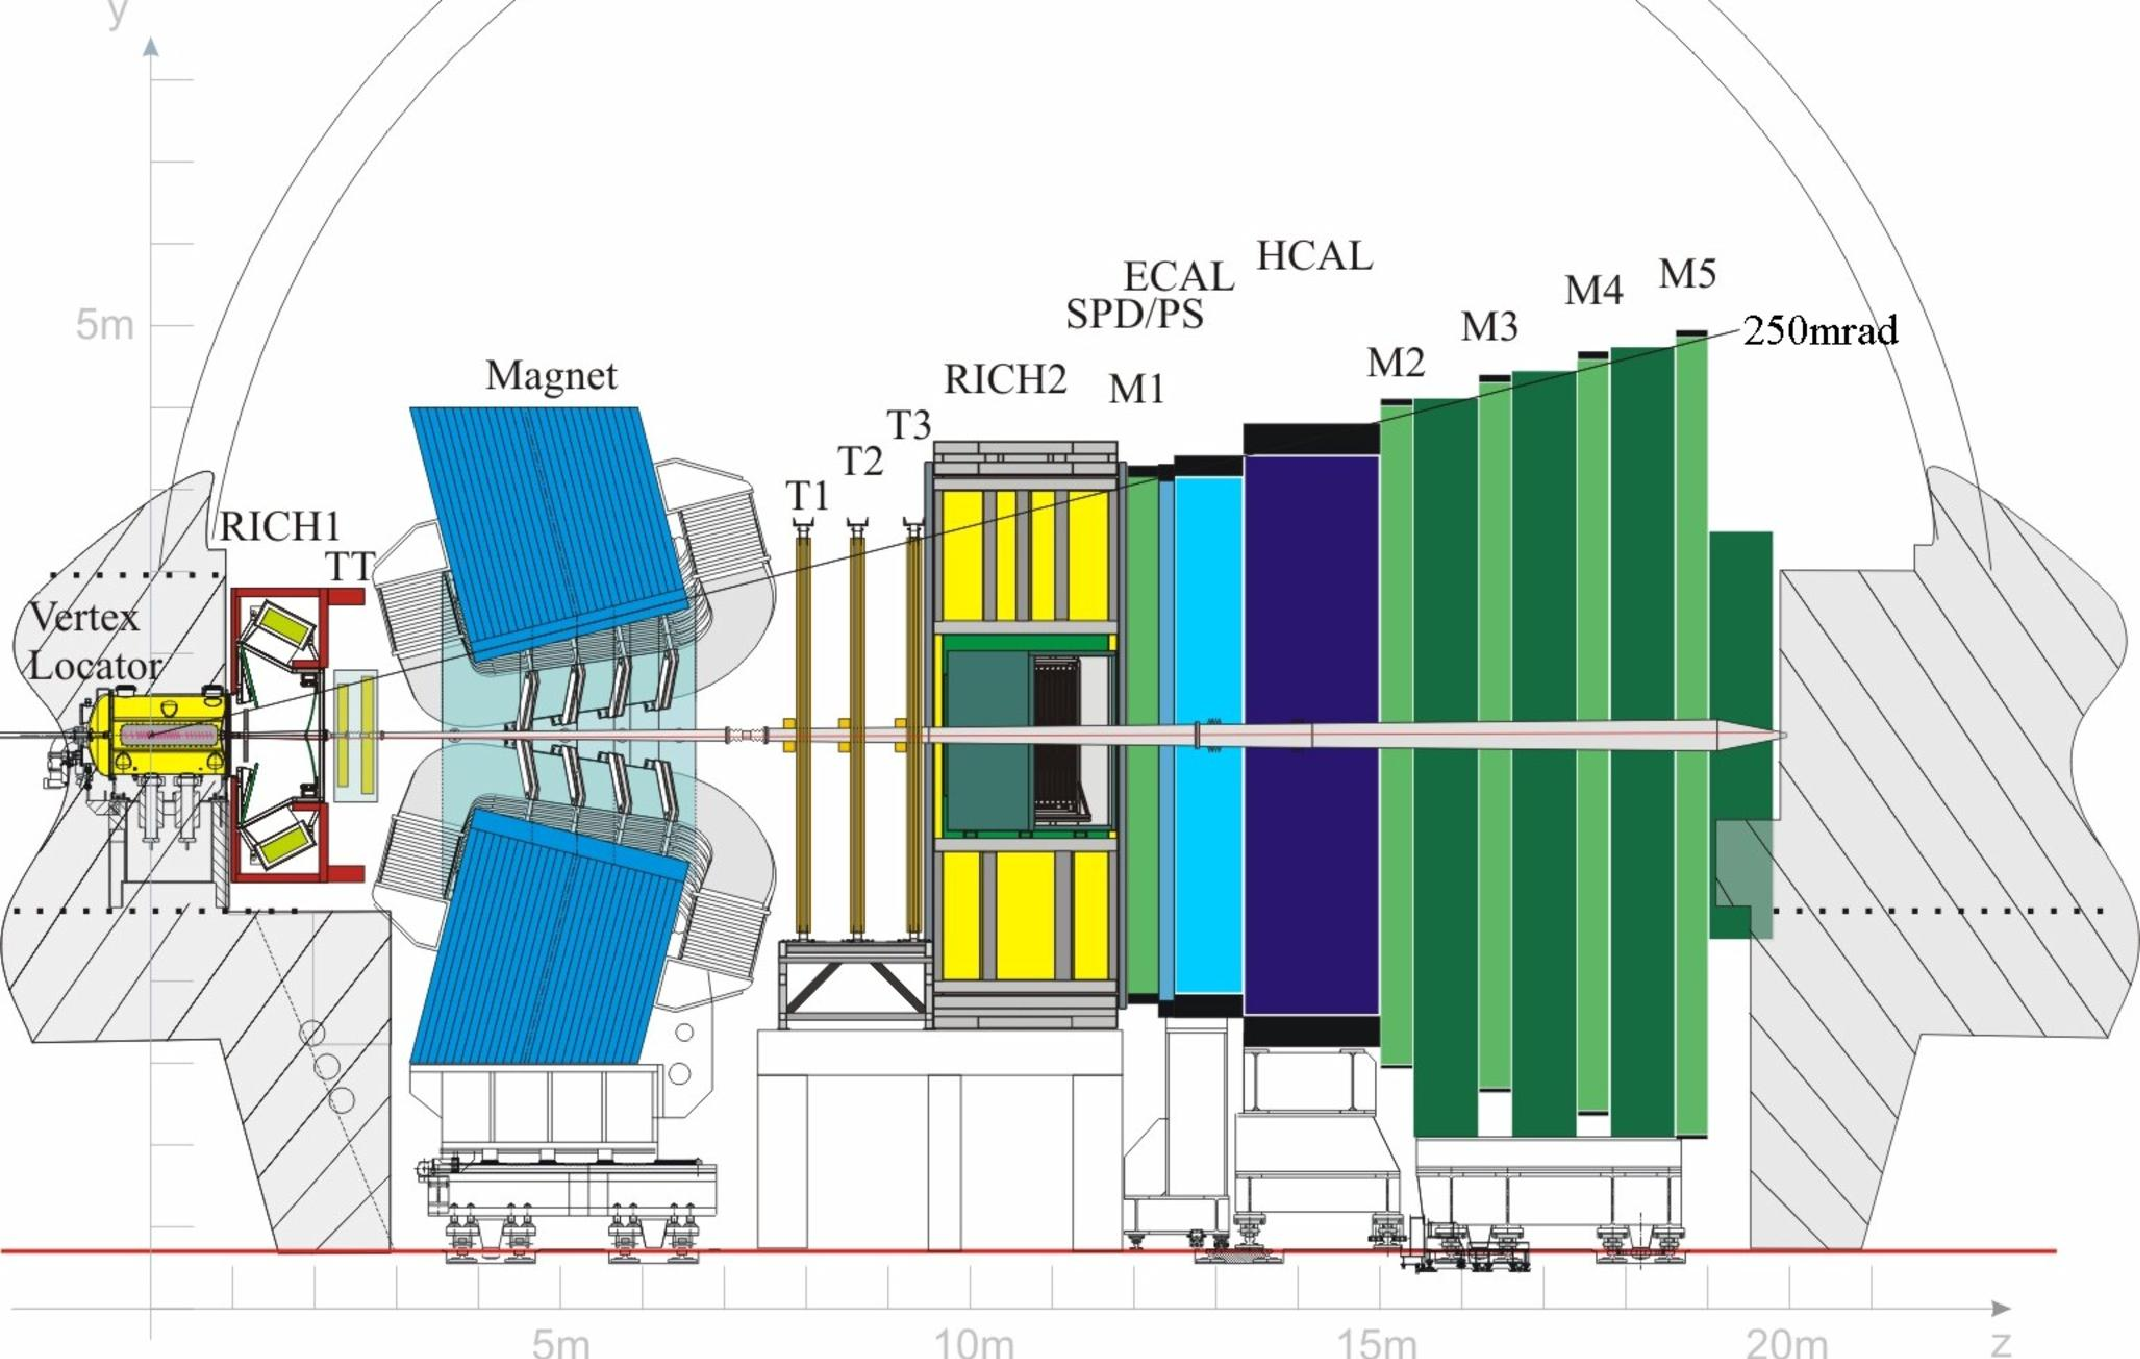
\includegraphics[width=0.7\linewidth]{images/LHCb_diagram.png}
    \caption{The LHCb Detector.}
    \label{LHCb}
\end{figure}

(Detector elements from left to right:  I-Vertex locator, II-Ring Imaging Cherenkov Detector 1, III-Trigger Tracker(TT), IV-Dipole Magnet, V-Outer Trackers(T1,T2 and T3), VI-Ring Imaging Cherenkov Detector 2, VII-Muon Detector 1, VIII-Electromagnetic and Hadronic Calorimeters, IX-Muon Detector 2,3,4 and 5).

The LHCb detector consists of several specialized subdetectors designed to reconstruct and identify particles produced in high-energy proton-proton collisions. At the heart of its tracking system is the VELO (Vertex Locator), which uses silicon-strip detectors positioned close to the beam line to provide precise reconstruction of primary and secondary vertices; it can be retracted during beam injection to protect it from damage. Upstream of the magnet is the TT Station (Trigger Tracker), a silicon microstrip detector that tracks particles before they enter the magnetic field. The dipole magnet itself generates an integrated magnetic field of about 4 T·m, bending the paths of charged particles so that their momenta can be measured downstream. Following the magnet, the tracking stations T1, T2, and T3, composed of straw tube drift chambers, continue to track the charged particles as they exit the magnetic field, ensuring accurate momentum measurement. For particle identification, Ring-Imaging Cherenkov Detectors (RICH) exploit the Cherenkov effect to distinguish between pions, kaons, and protons by measuring the angle of Cherenkov radiation, which is directly related to the particle’s velocity. The equation for the angle in terms of the velocity of the radiating particle is:
    \[
    \cos(\theta_{C}) = \frac{1}{n \frac{v}{c}} = \frac{c}{n v}
    \]
    where the \qq{$n$} is the refractive index of the detector material.
    \begin{figure}[H]
        \centering
        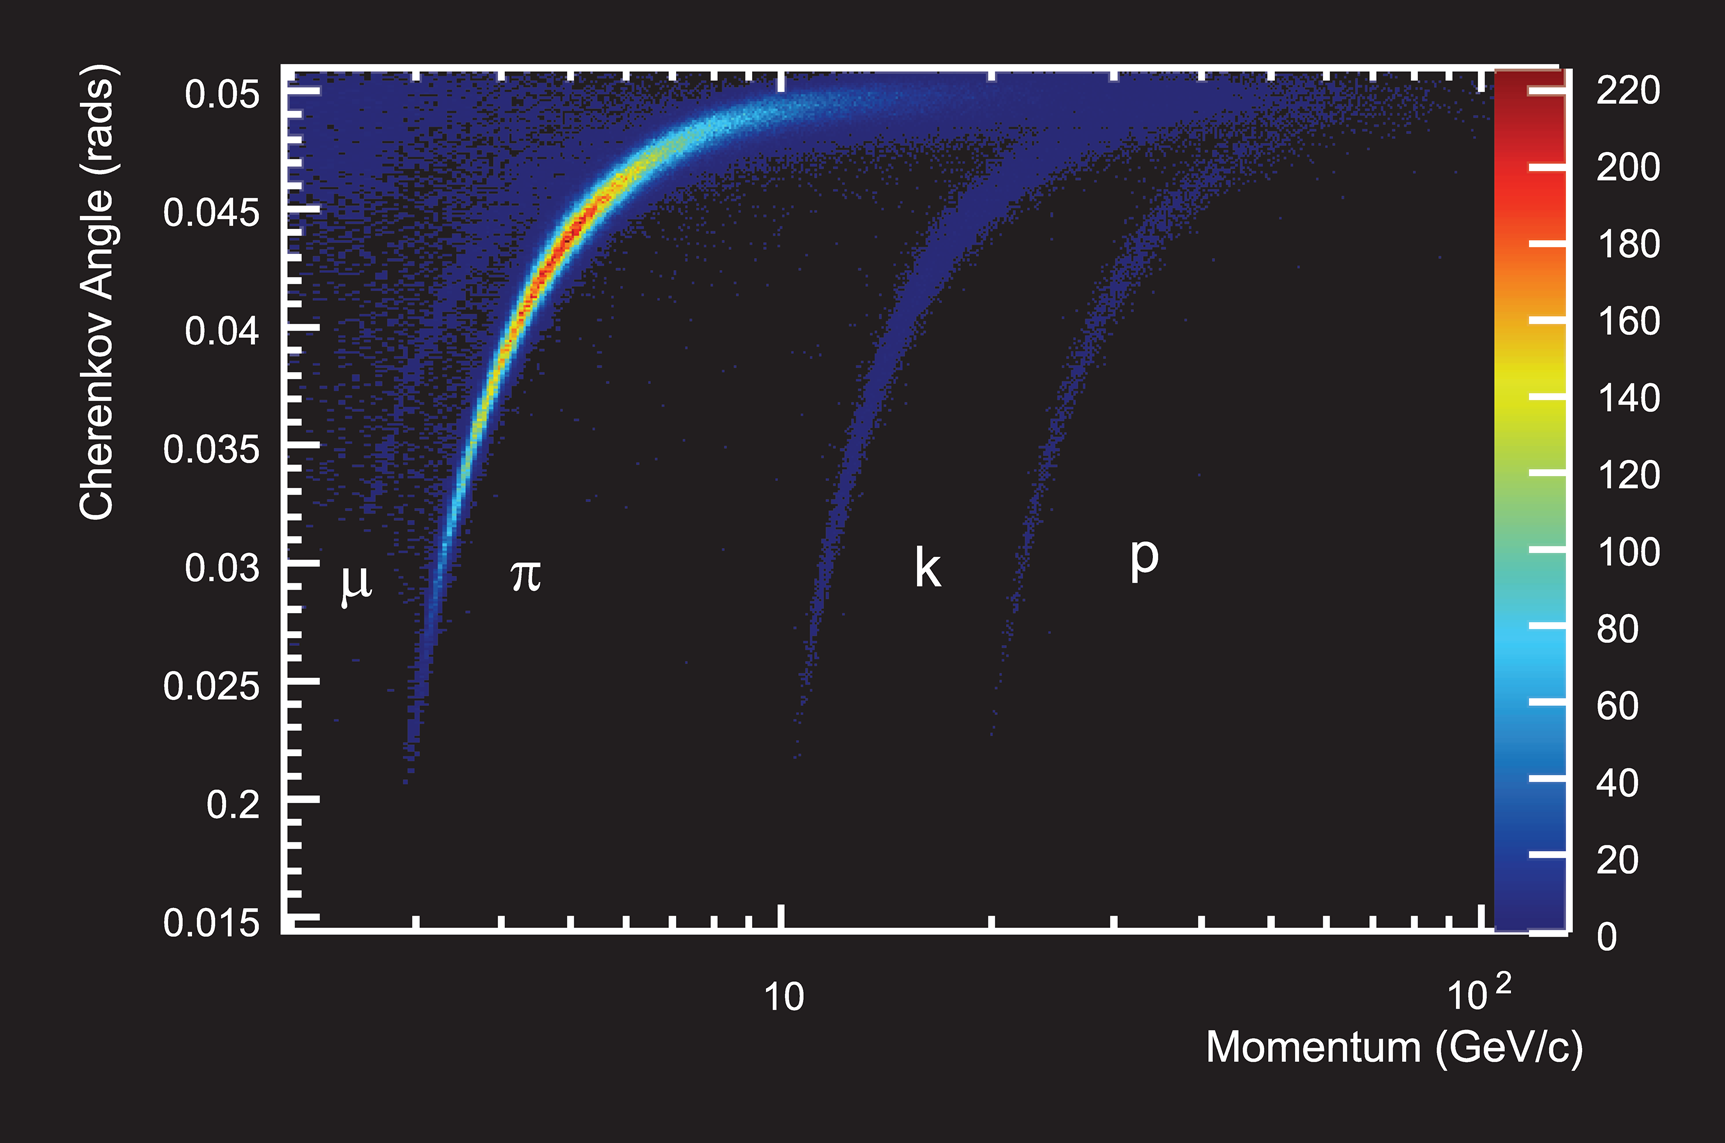
\includegraphics[width=0.59\linewidth]{images/RICH_ID.png}
        \caption{Possible particles and their momentum via a given Cherenkov angle.}
        \label{RICH}
    \end{figure}
    Complementing this system are the calorimeters, which measure the energy of electrons, photons, and hadrons through the development of particle showers. This calorimeter system includes a scintillating pad detector and preshower detector for electron/photon discrimination, an electromagnetic calorimeter for precise measurement of electrons and photons, and a hadronic calorimeter for measuring the energy of hadrons, including neutral hadrons like neutrons. Finally, the muon system, consisting of five stations (M1–M5) with multi-wire proportional chambers and gas electron multipliers, identifies muons, with M1 placed before and M2 to M5 positioned after the calorimeters, separated by shielding layers to suppress background. Together, these subsystems enable LHCb to perform precise measurements and probe fundamental questions in particle physics.
%--------------%
\newpage
\section{\texorpdfstring{Isolating the $B_{s}^{0}$}{} Decay}

In this laboratory course, we are interested in analysing the specific decay $B_s^0 \rightarrow \psi(2S)\,K_S^0$.
\begin{figure}[H]
    \centering
    \begin{tikzpicture}
        \begin{feynman}
            \vertex (a1) {\(\overline b\)};
            \vertex[right=1.5cm of a1] (a2);
            \vertex[right=1cm of a2] (a3);
            \vertex[right=1.5cm of a3] (a4) {\(\overline d\)};
            \vertex[below=2em of a1] (b1) {\(s\)};
            \vertex[below=2em of a4] (b2) {\(s\)};
            \vertex[above=2em of a4] (c1) {\(c\)};
            \vertex[above=2em of c1] (c2) {\(\overline c\)};
            \diagram* {
            (a4) -- [fermion] (a3) -- [boson, edge label=\(W^{+}\)] (a2) -- [fermion] (a1),
            (b1) -- [fermion] (b2),
            (c2) -- [fermion] (a2),
            (a3) -- [fermion] (c1),
            };
            \draw [decoration={brace}, decorate] (b1.south west) -- (a1.north west)
            node [pos=0.5, left] {\(B^{0}_{s}\)};
            \draw [decoration={brace}, decorate] (c2.north east) -- (c1.south east)
            node [pos=0.5, right] {\(\psi(2S)\)};
            \draw [decoration={brace}, decorate] (a4.north east) -- (b2.south east)
            node [pos=0.5, right] {\(K^{0}_{S}\)};
        \end{feynman}
    \end{tikzpicture}  
\caption{Leading order feynman diagram for the decay $B^{0}_{s} \xrightarrow{} \psi(2S)K^{0}_{S}$.}
\end{figure}

This decay is interesting to analyze because of some CP sensitive properties. However, it is also going to be vital to utilize the signal of the similar, but more abundant decay of $B_d^0 \rightarrow \psi(2S)\,K_S^0$ in our dataset.

\begin{figure}[H]
    \centering
    \begin{tikzpicture}
        \begin{feynman}
            \vertex (a1) {\(\overline b\)};
            \vertex[right=1.5cm of a1] (a2);
            \vertex[right=1cm of a2] (a3);
            \vertex[right=1.5cm of a3] (a4) {\(\overline s\)};
            \vertex[below=2em of a1] (b1) {\(d\)};
            \vertex[below=2em of a4] (b2) {\(d\)};
            \vertex[above=2em of a4] (c1) {\(c\)};
            \vertex[above=2em of c1] (c2) {\(\overline c\)};
            \diagram* {
            (a4) -- [fermion] (a3) -- [boson, edge label=\(W^{+}\)] (a2) -- [fermion] (a1),
            (b1) -- [fermion] (b2),
            (c2) -- [fermion] (a2),
            (a3) -- [fermion] (c1),
            };
            \draw [decoration={brace}, decorate] (b1.south west) -- (a1.north west)
            node [pos=0.5, left] {\(B_d^{0}\)};
            \draw [decoration={brace}, decorate] (c2.north east) -- (c1.south east)
            node [pos=0.5, right] {\(\psi(2S)\)};
            \draw [decoration={brace}, decorate] (a4.north east) -- (b2.south east)
            node [pos=0.5, right] {\(K^{0}_{S}\)};
        \end{feynman}
    \end{tikzpicture}
\caption{Leading order feynman diagram for the decay $B_d^{0} \xrightarrow{} \psi(2S)K^{0}_{S}$.}
\end{figure}
The data we receive, which has already been through a preliminary computer intensive selection process, is a reconstruction of the initial state of $B^{0}_{S}$ meson from the candidates of final state from the decay: $B_s^0 \rightarrow \psi(2S)\,K_S^0 \rightarrow (\mu^-\mu^+) (\pi^-\pi^+)$.

Our task is to isolate the signal of the $B_s^0$ decay from a combinatorial background LHCb dataset,in the following, we are going to explain how we trained a classifier to do that; so we need here to introduce and explain some theoretical concepts.

\subsection{Figure of merit and significance}

During the training procedure of the classifier we need to evaluate and optimize the performances, maximizing the number of signal candidates while keeping the background low.
In order to increase the performances we minimize the loss function: a function that measures the absolute value distance between the true target value and the one predicted by the classifier.

The inverse of such loss functions is called \qq{Figure of merit} (FOM). In this analysis, we use the Punzi FOM test to calculate the significance of the signal that comes out of our multivariate classifier:

\begin{equation}
    \text{FOM}=\frac{\epsilon_{\text{sig}}}{\frac{5}{2}+\sqrt{N_{\text{bkg}}}}
    \label{eq:punzi}
\end{equation}

where $N_{\text{bkg}}$ is the number of background events in the signal region and $\epsilon_{\text{sig}}$ is the classification efficiency of the signal.

After the optimal cut has been found, we need to evaluate the number of signal events in the data sample. To this end, we model the invariant mass distribution of the $\psi(2S)K_{S}$ combination with two peaks ($B_s^0$ and $B_d^0$ events) and a decreasing exponential function
for the remaining combinatorial background. By fitting this model to the data distribution, the number of signal candidates can be obtained from the integral of the signal peak model.

From here, we can also compute an estimated significance of the observation:

\begin{equation}
    m=\frac{N_{\text{sig}}}{\sqrt{N_{\text{sig}}+N_{\text{bkg}}}}
    \label{eq:sig}
\end{equation}
